\documentclass[10pt,a4paper,onecolumn,notitlepage]{scrartcl}

%%  Os pacotes da AMS devem ser carregados antes de fontenc e babel (Dica do Uma não tão pequena introdução ao LATEX 2ε)
\usepackage{amsmath}  
\usepackage{amsfonts}
\usepackage{amssymb}

\usepackage[utf8x]{inputenc} % compilando com o lualatex não precisa desta linha. lualatex é unicode por padrão.
\usepackage[brazil]{babel}
\usepackage[T1]{fontenc} % sem esse pacote a hifenização não funciona corretamente com palavras acentuadas.
\usepackage{ucs}
\usepackage{graphicx}
%\usepackage{wrapfig}
\usepackage[osf]{mathpazo}
%\usepackage[osf,sc]{mathpazo}
\usepackage{hyperref}
%\usepackage{layouts}
%\usepackage{scrpage2}
\usepackage{tikz}
\usepackage{multicol}
\usepackage{siunitx}
\usepackage{enumitem}
\usepackage{float}
\usepackage{fancyhdr}

\usepackage[textheight=24cm]{geometry}

%\renewcommand{\thesection}{\arabic{section}}
%\numberwithin{equation}{section}
\newcommand{\refeq}[1]{Equação \eqref{#1}}
\newcommand{\HRule}{\rule{\linewidth}{0.5mm}}

\author{}
\title{Prática 3: Pêndulo Simples}


%\thispagestyle{myheadings}
\pagestyle{fancy}
\lhead{}
\chead{}
\rhead{\textsc{Prática 3: Pêndulo Simples}}
\cfoot{\thepage}
\renewcommand{\headrulewidth}{0.4pt}

%\setcounter{tocdepth}{1} % Profundidade do sumário: 0 - mostra apenas os capítulos.

\begin{document}
\thispagestyle{myheadings}

\begin{figure}
\begin{minipage}{0.08\linewidth}
\includegraphics[scale=0.5]{figuras/brasaoUFC.jpg} 
\end{minipage}
\begin{minipage}{0.91\linewidth}
\textsc{Universidade Federal do Ceará}

Disciplina: EM0016 - Física Experimental para Engenharia
\end{minipage}

\begin{minipage}{\linewidth}
%\vspace{0.1cm}
\centering
\textsc{Prática 3: Pêndulo Simples}
\\
\hrulefill % usar este comando quando não estiver dentro de uma tabela.
\end{minipage}
\end{figure}

\section{Objetivos}

\begin{itemize}
\item Verificar experimentalmente as leis do pêndulo  e  determinar a aceleração da gravidade local.
\end{itemize}

\section{Material}

\setlist[1]{itemsep=-5pt}
\begin{multicols}{3}
\begin{itemize}
\item Massas  aferidas;
\item Cronômetro;
\item Fios;
\item Transferidor;
\item Coluna graduada.
\end{itemize}
\end{multicols}

\section{Fundamentos}
O pêndulo simples é o sistema constituído por uma massa puntiforme, presa à extremidade de uma fio extensível e de massa desprezível, capaz de se mover, sem atrito, num plano vertical, em torno de um eixo situado em sua outra extremidade. Pela própria definição, vemos que o pêndulo simples é uma concepção ideal. O que montaremos é aproximadamente um pêndulo simples.
\begin{figure}[ht]
\centering
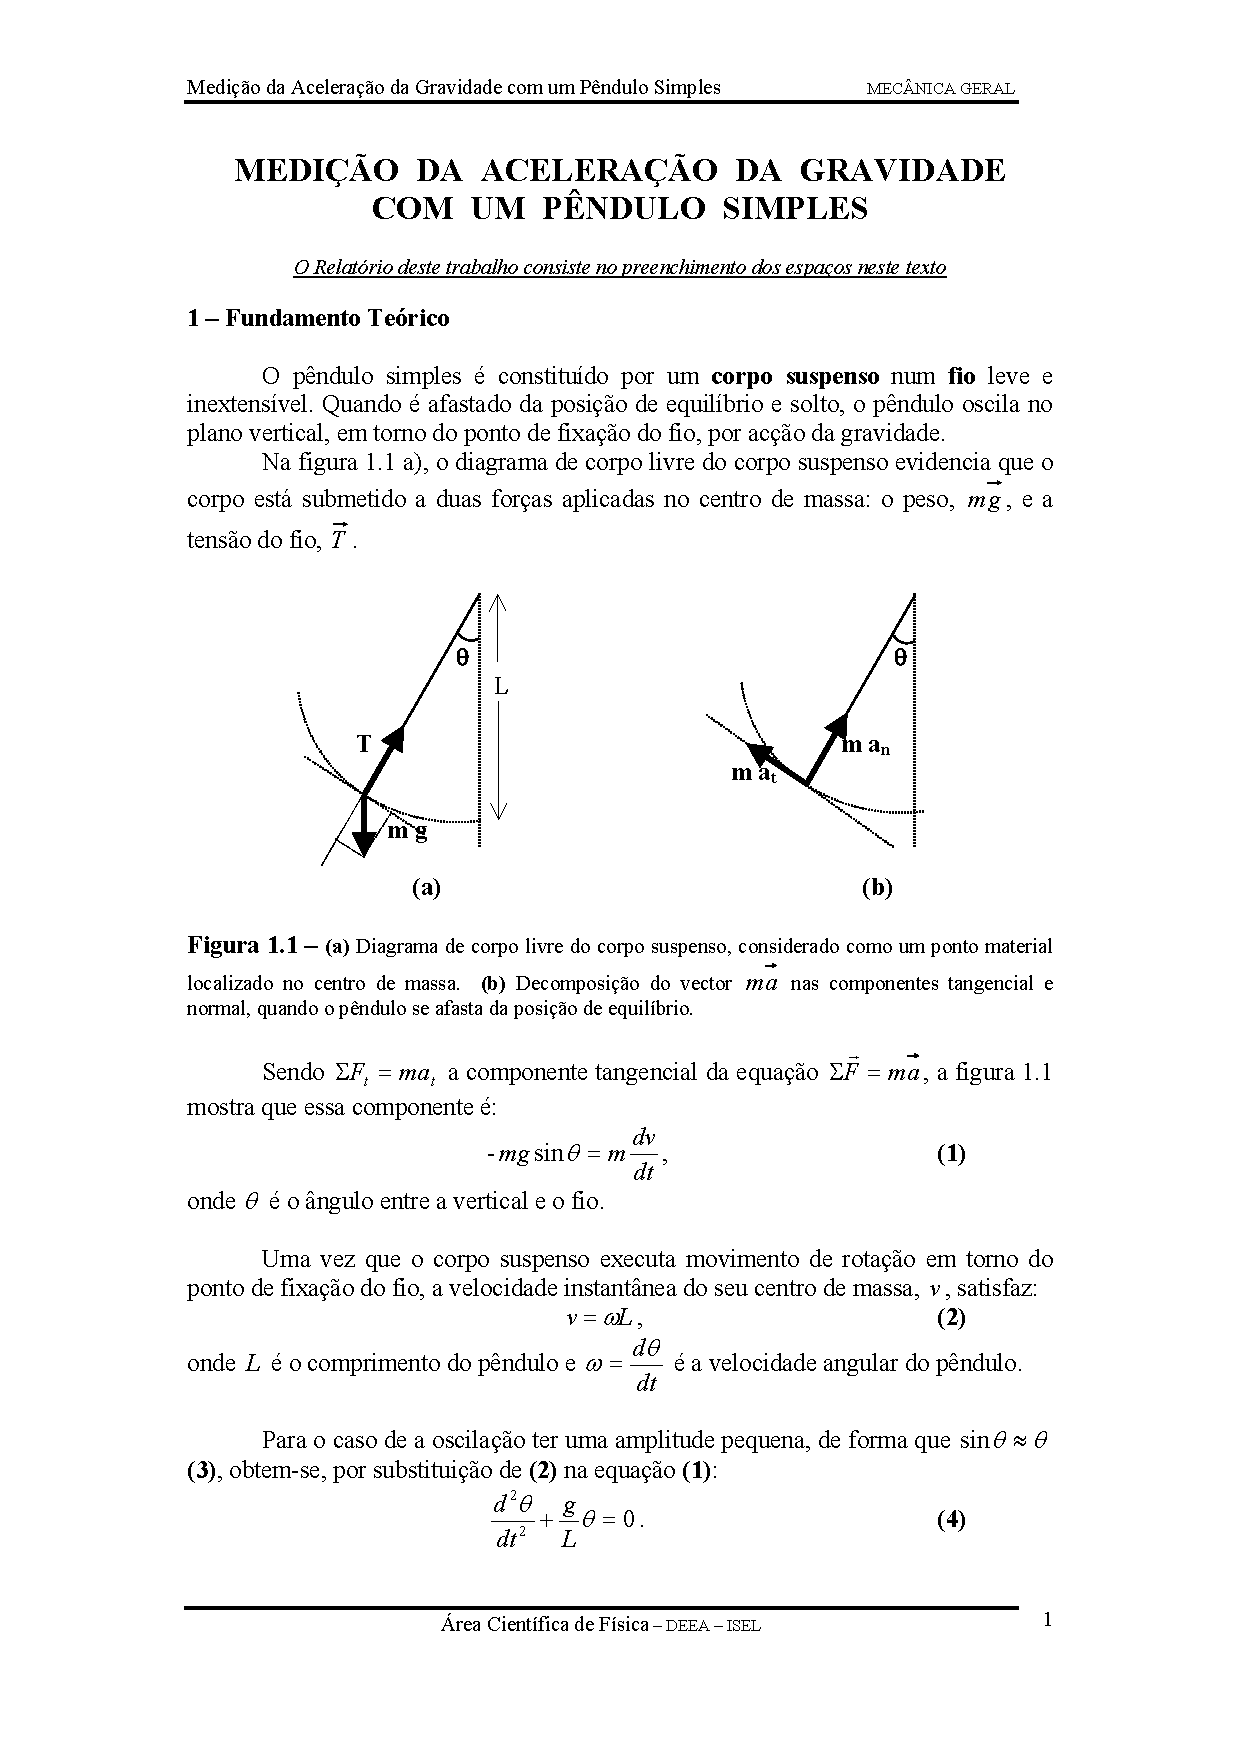
\includegraphics[scale=0.2]{figuras/pendulo/pendulo.png} 
\caption{Pêndulo simples}
\label{fig:pendulo}
\end{figure}

Quando afastada da posição de equilíbrio e solto, o pêndulo oscila sob a ação da gravidade.  O movimento é oscilatório e periódico. Numa posição qualquer, afastada de um ângulo $\theta$ da posição de equilíbrio, as forças aplicadas à massa são:  $mg$ (peso)  e  $T$ (tração  no  fio). Decompondo o peso conforme indica a Figura \ref{fig:pendulo}, obtemos as componentes $mg \cos\theta$ e $mg \sin\theta$. A resultante da tração e $mg \cos\theta$  produz  a  aceleração  centrípeta.  A  outra  componente,  $mg \sin\theta$,  é  a  força  restauradora  que  age  sobre  $m$.  Ela  não  é  proporcional  à  alongação  $\theta$   e  sim  a  $\sin\theta$,

\begin{align}
F = -mg\sin\theta
\label{eq:forca-prop}
\end{align}

Para que o movimento seja harmônico simples é necessário que a força restauradora seja proporcional ao deslocamento e dirigida no sentido oposto.

Podemos substituir $\sin\theta$ por $\theta$, caso $\theta$ seja pequeno. Esta aproximação é válida para $ \theta < \frac{\pi}{12} rad$ ($\theta < 15^{o}$)

Na Figura \ref{fig:pendulo} podemos ver que: $\overline{AB} = \theta L$, ou $\theta = \frac{\overline{AB}}{L}$, logo,
\begin{align}
F = -mg(\frac{\overline{AB}}{L})
\end{align}

Assim, no caso de pequenas oscilações, a força restauradora é proporcional e de sentido oposto à elongação medida sobre o arco considerado retilíneo. Note que esta é, exatamente, a característica do movimento harmônico simples.

Como $m$, $g$ e $L$ são constantes, podemos expressá-las por
\begin{align}
k = \frac{mg}{L}
\label{eq:constanteelastica}
\end{align}

Temos então:

\begin{align}
F = -kx
\label{eq:forca}
\end{align}

Sabemos que o período $T$, de um movimento harmônico simples é dado por:

\begin{align}
T = 2\pi\sqrt{\frac{m}{k}}
\label{eq:periodo}
\end{align}

Substituindo o valor de $k$, Equação \ref{eq:constanteelastica}, na equação \ref{eq:periodo}, temos:
\begin{align}
T=2\pi\sqrt{\frac{L}{g}}
\label{eq:periodo2}
\end{align}

que é a equação do período do pêndulo simples, para pequenas amplitudes. Vemos daí que o período de um pêndulo simples depende apenas do comprimento do pêndulo e do valor da aceleração da gravidade.

\subsection{Determinação Experimental da Aceleração da Gravidade~($g$)}

Elevando ao quadrado a Equação \ref{eq:periodo2}, vem:
\begin{align}
T^2=4\pi^2\frac{L}{g}
\end{align}

Depois de medir o comprimento $L$ e o período $T$ do pêndulo, podemos facilmente calcular o valor da acelaração da gravidade $g$. Basta isolar $g$ na \ref{eq:periodo2}. 

\begin{align}
g=4\pi^2\frac{L}{T^2}
\label{eq:valordeg}
\end{align}

\section{Procedimento Experimental}
\setlist[1]{itemsep=2mm}
\begin{enumerate}
\item Anote as massas dos corpos $m_1$ e $m_2$.
\item Ajuste o comprimento do pêndulo de modo que tenha $20cm$ de extensão do ponto de suspensão até o centro de massa do corpo.
\item Desloque o corpo da posição de equilíbrio (deslocamento angular igual a $15^o$) e determine o tempo necessário para o pêndulo executa dez oscilações completas. Para minimizar os erros, é recomendável que o operador do cronômetro seja o mesmo que larga o pêndulo para oscilar.
\begin{quote}
Obs.: O tempo de reação humano é de alguns décimos de segundo; Embora o cronômetro registre até centésimos de segundo, só faz sentido você anotar o tempo obtido manualmente até os décimos de segundo.
\end{quote}
Repita o experimento três vezes e determine o período médio em segundos. Use somente a massa $m_1$ como indicado na Tabela \ref{tab:tabm1} na página \pageref{tab:tabm1}.

\item Repita a experiência para os comprimentos $40cm$, $60cm$, $80cm$, $100cm$, $120cm$ e $140cm$ e complete a Tabela \ref{tab:tabm1}.

\item Mantenha o comprimento de $140cm$ e estude a influência da massa e da amplitude sobre o período. Proceda como indicado na Tabela \ref{tab:massaamplitude}.

\end{enumerate}

\begin{table}
\centering
\renewcommand{\arraystretch}{1.5}
\begin{tabular}{|l|l|p{15mm}|p{15mm}|p{15mm}|p{15mm}|p{15mm}|p{15mm}|}
\hline
$L(cm)$ & $\theta (graus)$ & $m (g)$ & \multicolumn{3}{c|}{$10T (s)$}  & $T(s)$ & $T(s^2)$ \\
\hline
\hline
$L_1 = 20 $ & $\theta_1 = 15$ & $m_1 = $ & $10T_1 = $ & $10T_1 = $& $10T_1 = $& $T_1 = $ & $T_1^2 = $ \\
\hline
$L_2 = 40 $ & $\theta_1 = 15$ & $m_1 = $ & $10T_2 = $ & $10T_2 = $& $10T_2 = $& $T_2 = $ & $T_2^2 = $ \\
\hline
$L_3 = 60 $ & $\theta_1 = 15$ & $m_1 = $ & $10T_3 = $ & $10T_3 = $& $10T_3 = $& $T_3 = $ & $T_3^2 = $ \\
\hline
$L_4 = 80 $ & $\theta_1 = 15$ & $m_1 = $ & $10T_4 = $ & $10T_4 = $& $10T_4 = $& $T_4 = $ & $T_4^2 = $ \\
\hline
$L_5 = 100 $ & $\theta_1 = 15$ & $m_1 = $ & $10T_5 = $ & $10T_5 = $& $10T_5 = $& $T_5 = $ & $T_5^2 = $ \\
\hline
$L_6 = 120 $ & $\theta_1 = 15$ & $m_1 = $ & $10T_6 = $ & $10T_6 = $& $10T_6 = $& $T_6 = $ & $T_6^2 = $ \\
\hline
$L_7 = 140 $ & $\theta_1 = 15$ & $m_1 = $ & $10T_7 = $ & $10T_7 = $& $10T_7 = $& $T_7 = $ & $T_7^2 = $ \\
\hline
\end{tabular}
\caption{Resultados experimentais para o pêndulo simples.}
\label{tab:tabm1}
\end{table}

\begin{table}
\centering
\renewcommand{\arraystretch}{1.5}
\begin{tabular}{|l|l|p{15mm}|p{15mm}|p{15mm}|p{15mm}|p{15mm}|p{15mm}|}
\hline
$L(cm)$ & $\theta (graus)$ & $m (g)$ & \multicolumn{3}{c|}{$10T (s)$}  & $T(s)$ & $T(s^2)$ \\
\hline
\hline
$L_7 = 140 $ & $\theta_1 = 15$ & $m_1 = $ & $10T_7 = $ & $10T_7 = $& $10T_7 = $& $T_7 = $ & $T_7^2 = $ \\
\hline
$L_8 = 140 $ & $\theta_2 = 10$ & $m_1 = $ & $10T_8 = $ & $10T_8 = $& $10T_8 = $& $T_8 = $ & $T_8^2 = $ \\
\hline
$L_9 = 140 $ & $\theta_1 = 15$ & $m_2 = $ & $10T_9 = $ & $10T_9 = $& $10T_9 = $& $T_9 = $ & $T_9^2 = $ \\
\hline
$L_10 = 140 $ & $\theta_2 = 10$ & $m_2 = $ & $10T_{10} = $ & $10T_{10} = $& $10T_{10} = $& $T_{10} = $ & $T_{\text{10}}^\text{2} = $ \\
\hline
\end{tabular}
\caption{Resultados experimentais para o pêndulo simples.}
\label{tab:massaamplitude}
\end{table}

\section{Questionário}
%\setlist[1]{itemsep=0mm}
\begin{enumerate}
\item Dos resultados experimentais  é  possível  concluir-se  que  os  períodos  independem  das  massas?  Justifique.
\item Dos resultados experimentais o que se pode concluir sobre os períodos quando a amplitude passa de $10^o$ para $15^o$? Justifique.
\item Determine o valor de $g$ a partir da Equação \ref{eq:valordeg}.
\item Qual o peso de um objeto de massa $9,00kg$ no local onde foi realizada a experiência?
\item Compare  o  valor médio  de  $T$  obtido  experimentalmente  para  $L = 140 cm$  com  o  seu  valor  calculado  pela  Equação \ref{eq:periodo}  (use $g = 9,81 m/s^2$). Comente.
\item Discuta  as  transformações  de  energia  que  ocorrem  durante  o  período  do  pêndulo.
\item Chama-se  \emph{pêndulo  que  bate  o  segundo}  aquele  que  passa  por  sua  posição  de  equilíbrio,  uma  vez  em  cada  segundo.  Qual  o  período  deste  pêndulo?
\end{enumerate}

\end{document}